
%%% Local Variables: 
%%% mode: latex
%%% TeX-master: t
%%% End: 

\chapter{相关工作}
\section{Web Service相关研究概述}
Web服务从广义上指基于网络的主机与主机之间互操作的软件系统。Web服务的主要特点在于提供轻量级的Web调用接口提供自足的(self-contained)松耦合的服务。狭义Web服务特指Web Service类似于W3C制定的基于SOAP协议的服务架构。该架构最基本的元素如引言所述的SOAP+WSDL+UDDI。关于Web Service架构的研究与应用开发在21世纪伊始比较热,而最近大与服务提供商更加倾向于使用形式上更加简单的REST接口。
\subsection{基于SOAP协议的Web Service}
\subsubsection{服务架构}
与工业界注重W3C及企业联盟注重标准制定与协议规范不同,学术界更加注重以通信协议为基础如何解决在资源动态变化的基础上解决日益复杂的应用需求。研究的问题主要包括Web数据集成、服务组合、访问控制、事件机制以及语义网(semantic web)相关研究。一个最基本的Web Service架构如图\ref{fig:web-service-arc-2}所示。

\begin{figure}[H]
  \centering
  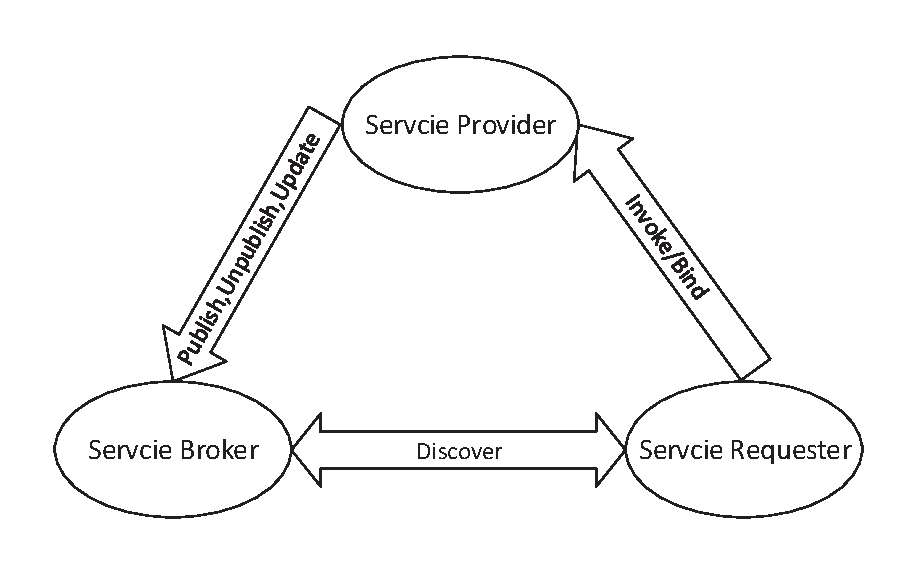
\includegraphics[width=0.6\textwidth]{web-service-arc-2}
  \caption{Web Service模型架构}
  \label{fig:web-service-arc-2}
\end{figure}

Bussler\cite{fensel2002web}指出由UDDI,WSDL和SOAP组成的协议栈无法实现真正可扩展的广域Web Service服务。实现可扩展的Web服务发现,选择,协调以及组合需要包含以下最基本的元素\cite{bussler2001b2b}:
\begin{itemize}
\item 文档类型(Document Types):文档类型为交换文档的基本语义。即文档类型定义了服务请求者与服务提供者数据交换的格式以及需要采取的语义(semantics)。
\item 语义(semantics):服务提供者与服务请求者确定相同的文档类型并保证传递信息语义的正确。因此需要语义词典来枚举文档元素所有可能的可用值。本体论(ontology)提供了一种对数据概念定义的一种手段,以保证对于数据概念解释的一致性。
\item 相关传输协议:服务请求双方需要约定好一致的通信协议。针对SOAP协议,底层协议可以为HTTP,SMTP,TCP,UDP或者JMS。
\item 信息交换序列:由于底层交换信息未必是可靠传输,可能发生报文重传与丢失现象,所以需要对交换报文添加序列号或消息确认以保证交换信息的完整性。
\item 流程:对于一个完整的服务而言,一次服务信息交换未必能够完成指定服务。例如一次购买行为,需要先将商品加入购物车,确定订单之后付款。之间至少需要三次服务请求双方的信息交换,并且顺序不能颠倒。所以服务双方需要确定一套服务协议流程。
\item 安全:安全性即服务最基本的需求,包括保证报文的私密性以及完整性。再次基础上还有服务与资源的访问控制等问题
\item 句法:即文档格式,如XML,JSON等
\item 服务配置:在各个相关服务端进行交互之前,可能服务主机的配置不相同,例如语义词典,服务流程等。当双方开始进行交互时,需要根据服务端进行特定配置。
\end{itemize}

文献\cite{fensel2002web}提出Web服务建模框架(Web Service Modeling Framework,WSMF)。WSMF旨在提出一套完全灵活并可扩展的Web服务架构。W3C也以WSMF框架为基础发布了一些列Web Service规范。\cite{WSMF-imp}WSMF架构。WSMF架构基于一下两个原则:元件,元素之间的强解耦性;强中介性,任何元素或服务之间可以通过扩展方式进行相互对话,强调元素与目标的的重用性及语义。WSMF的十字形架构如图\ref{fig:WSMF-arc}所示。图\ref{fig:WSMF-arc}采用文献\cite{WSMF-imp}的改进“十字形模型”。

\begin{figure}[H]
  \centering
  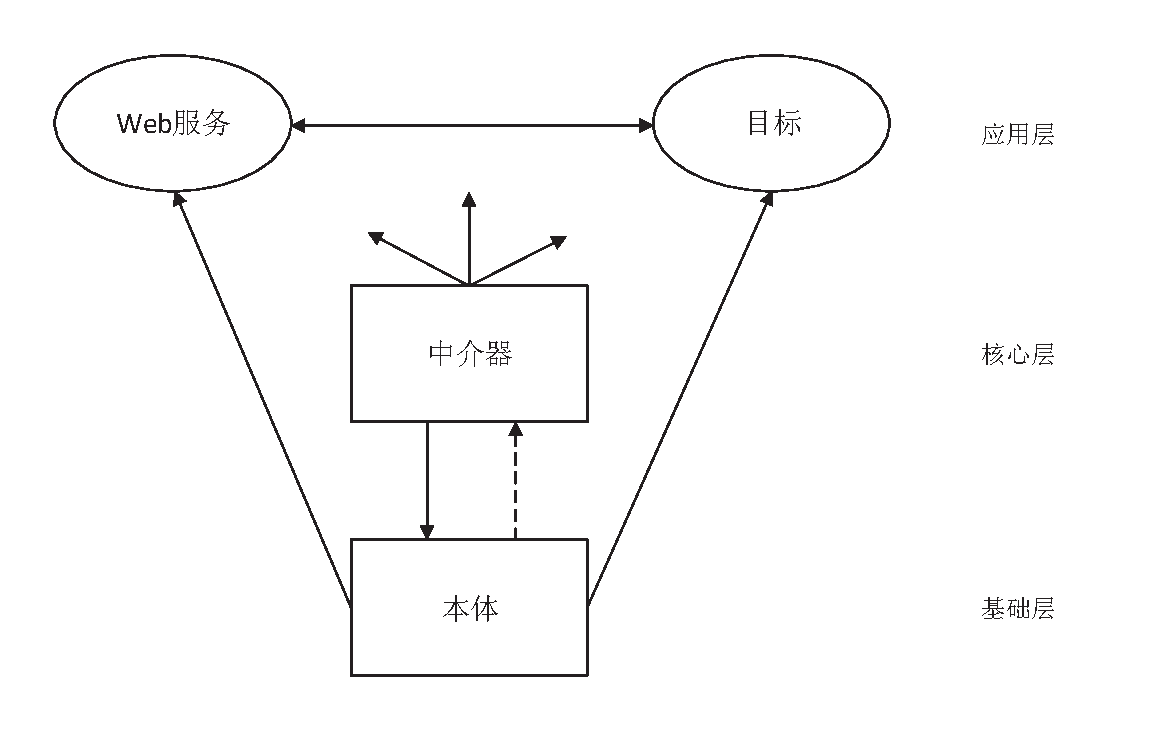
\includegraphics[width=0.7\textwidth]{WSMF-arc}
  \caption{WSMF顶层要素与相互关系}
  \label{fig:WSMF-arc}
\end{figure}

该模型中应用层为各种可被重用的任务集$\{\mathrm{WS}\mid\mathnormal{ws_{1}}, \mathnormal{ws_{2}}, \mathnormal{ws_{3}} \cdots \mathnormal{ws_{m}}\}$ 与$ \{\mathrm{G}\mid\mathnormal{g_{1}}, \mathnormal{g_{2}}, \mathnormal{g_{3}} \cdots \mathnormal{g_{n}}\}$。在具体实现相关应用时即为实现指定目标$\mathnormal{G_j}, \mathnormal{G_j}\subset\mathnormal{G}$而按一定流程重新组合$\mathnormal{W_i}, \mathnormal{W_i}\subset\mathnormal{W}$。

WSMF的核心为中介器,包括本体中介器,目标中介器,服务中介器,以及目标服务组着中介器。用来协调各个元素之间的组合关系。此外需要协调服务与服务之间包括传送协议,数据结构,信息格式的不同方言等问题。本体为WSMF架构的基础,对服务,目标,中介器进行描述和条件约束。

\subsubsection{服务发现}
在服务发现技术方面,服务发现是指服务请求者基于某单一既定目标查找选定需要的服务。工业界最常见的为UDDI服务,但依旧在更高的复杂性和信息组合自动化方面有所不足。当前Web服务发现的主要技术如表\ref{tab:web-service-discovery}所示。\cite{klein2001serching}

\begin{table}[htb]
  \centering
  \begin{minipage}[t]{0.8\linewidth}
  \caption{主流服务发现技术比较}
  \label{tab:web-service-discovery}
    \begin{tabular}{c	c	c	c}
      \toprule[1pt]
      \textbf{Service Discovery Technologies} & \textbf{Precision} & \textbf{Recall} & \textbf{Hardness} \\\midrule[0.5pt]
      Keyword Based & Low & High & Average\\
      Frame Based & High & Low & Average\\
      Deductive Retieval & High & High & Hard\\
      \bottomrule[1pt]
    \end{tabular}
  \end{minipage}
\end{table}

大多数检索方法是类似于基于UDDI的框架(Frame Based)方法。基于逻辑推导(Deductive Retieval)的方法由于服务在概念上与约束上非常难表述,所以实现难度最高。Mark Klein,Abraham Bernstein提出一套基于Ontology的服务发现架构,将服务描述通过语义网(Semantic Web)重新组织,提出了一套查询方式更加灵活,查询准确性更高的框架。\cite{klein2001serching}

\subsubsection{Web服务安全}
Web服务安全研究主要分为两个方面即,访问控制与数据安全。Web Service访问控制技术大体分为:
\begin{itemize}
\item 基于主机认证:基于访问主机请求中的网络认证信息(如hostname, IP等),缺点是无法控制区分同一主机的不同用户,信息也比较容易伪造。
\item 基本认证:基于辨识身份的用户名与密码,用户名与密码在基于HTTP的传输中保持为明文。
\item 基于SSL/TLS的身份证书:利用证书对传输信息进行加密或签名,是工业实现中相对可靠,并且主流的实现方式。而对证书的分发与信任模型(trust model)本身为密码工业的研究范围
\end{itemize}

WS-Security作为SOAP的扩展协议由OASIS于2002年提出。\cite{nadalin2002web}该协议旨在保证Web服务信息传输的加密型以及防止信息篡改。该协议支持多种安全信令包括X.509,Kerberos,以及 Security Assertion Markup Language(SAML),提供端到端的信息安全保护。

\subsection{基于REST的Web服务架构}
REST(表述性状态转移,Representational state transfer)不是指具体的某个协议,而是一种构建分布式可扩展web服务的最佳实践原则。REST通常通过HTTP协议来组织超媒体(Hypermedia)资源。

REST的主要设计原则为:
\begin{itemize}
\item 统一接口:通过HTTP动词(GET,POST,PUT,DELETE)对以URI标记的资源进行操作以代表创建,读取,更新,删除等操作
\item 自描述性:资源与其描述为松耦合,因此资源可以以不同的格式存在(XML,JPEG,PDF等)。客户端与服务端可以利用HTTP中对资源描述的元数据对资源进行操作
\item 无状态性:对于资源操作在服务端与客户端是无状态的。状态描述被显式的保存在超链接上。
\end{itemize}
以微信公共账号服务接口为例,采用REST风格的调用接口。通过服务号群发消息的接口如下:

\noindent
\fbox{
\parbox{0.9\textwidth}{
  \small{http请求方式: POST\\
  https://api.weixin.qq.com/cgi-bin/media/uploadnews?access\_token=ACCESS\_TOKEN}
 }
}

HTTP报文封装的POST的数据为JSON格式的一段文档。

一些组织也在进行基于REST的服务架构标准化工作,包括Open Mobile Alliance(OMA)以及IETF。OMA研究主要集中在基于Parlay-X(一种电话网络中Web Service的服务架构)REST接口研究与制定。\cite{alliancerestful}IETF也在制定基于REST的集中会议控制协议(Centralized Conferencing Manipulation Protocol,CCMP)\cite{barnes2009centralized}。

\section{信息中心网络相关研究概述}
\subsection{信息中心网络研究概述}
TCP/IP在早在20世纪70年代就被提了出来,当时网络的主要需求即为固定主机间端到端的可靠通信。且在简单IP层的瘦腰网络架构支持下,上层网络应用只要基于最简单的IP协议,即可在互联网上运行,所以大量的互联网创新应用随之而来。随着当今互联网越来越向数据分发的方向演进,以命名数据取代IP网络瘦腰的信息中心网络设计思想作为一种全新的架构被提出来。当前主要的ICN架构包括DONA,NDN,PRISP和NetInf。ICN设计主要考虑如下五个方面\cite{xylomenos2014survey}:

\begin{itemize}
\item 命名:在所有的ICN架构中,网络包的命名与主机地址无关。命名方式有两种,即扁平化或层次化的命名方式
\item 名字解析与数据路由:主要分为耦合和解耦两种方式。在耦合方式中,命名数据请求被转发到相应的主机后,数据沿着请求反向路径返回给数据请求者。在解耦方式中,数据应答的返回路径不做限制。
\item 缓存:缓存设计主要分为\textit{on-path}和\textit{off-path}两种。\textit{on-path}方式指的是数据被缓存在数据请求的转发路径上。\textit{off-path}缓存需要请求转发与路由系统支持,即缓存数据主机可以被当做正常的数据发布者
\item 移动:ICN天然地支持数据请求者的移动性,因为当请求链接失败之后,请求者可以在新的地点构建新的数据请求路径。而数据发布者的移动性支持较难,需要一定的路由机制重新更新请求路由转发表。
\item 安全:安全机制设计与数据命名方式直接相关。扁平的命名方式需要命名数据能够自验证,而结构化的命名方式则可以建立结构化的信任模型(trust model)。
\end{itemize}

\subsection{命名数据网络架构及研究进展}
本文中的命名服务网络设计主要基于ICN中的命名数据网络架构设计(Named Data Networking,NDN)。NDN架构在2009年由Van Jacobson等人提出。\cite{jacobson2009networking}NDN架构如图\ref{fig:IP-vs-NDN}所示。NDN的网络架构继承了IP架构的沙漏型瘦腰结构。由于瘦腰的简单性,上下层协议只要支持瘦腰协议即可进行大量创新,这个瘦腰架构也是互联网发展30年来的成功经验
。在NDN架构中利用命名数据包来取代以端主机地址标记的IP网络包。

\begin{figure}[H]
  \centering
  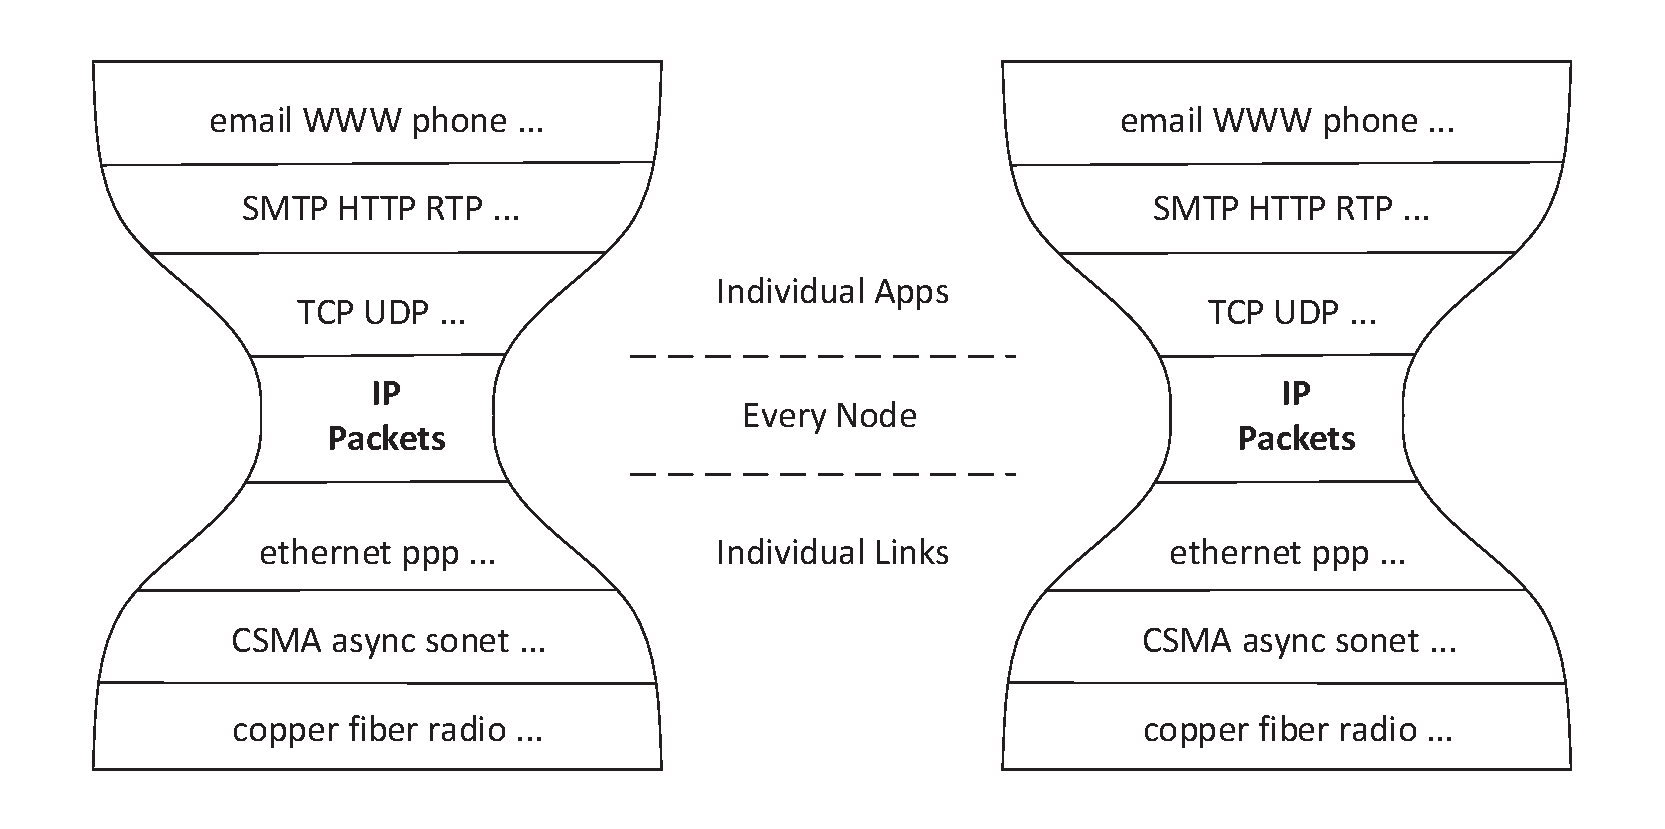
\includegraphics[width=0.9\textwidth]{IP-vs-NDN}
  \caption{IP与NDN架构对比}
  \label{fig:IP-vs-NDN}
\end{figure}

NDN的主要设计原则是:
\begin{itemize}
\item 命名:NDN采用结构化URI方式的命名。结构化的命名方式可以使路由更加具有扩展性,即可以采用名字前缀方式进行路由。命名方式不涉及网络上的信息如(IP地址)而是直接应用相关,即应用可以不依赖网络选择特定的命名方式。
\item 安全:安全特性在NDN架构的另一个基础。NDN架构采用以数据为中心的安全,及对每一个数据包单独进行签名。数据的安全性与数据在哪里存放解耦。
\item 名字解析与数据路由:名字解析不直接整合在NDN架构中,就像IP网络中DNS是独立的网络一样。NDN路由采用耦合方式,即数据会根据数据数据请求的转发路径反向转发。由于NDN采用前缀转发的方式与IP类似,所以NDN可以采用IP类似的BGP,IS-IS和OSPF转发协议。
\item 缓存:由于NDN采用耦合方式转发数据请求,数据可以被缓存在数据请求路径的中间节点上。而NDN与IP不同的是可以做到真正的网络层缓存。因为NDN数据包与IP数据包不同的是直接以应用数据名字命名,而不是以地址命名,所以在缓存中的数据可以被其他请求端重用。而由于NDN数据包的数据中心安全性,数据包缓存在网络中可以被加密也可以签名防止被篡改。
\item 智能数据平面:与IP不同,IP是一个无状态协议,路由器很难在IP的层面对路由状态进行监控。而NDN中的请求等待表(Pending Interest Table,PIT)记录了所转发数据请求的一些列转发状态信息。而抓发节点可以根据PIT所记录的软状态(soft state)构建智能的转发策略。
\end{itemize}

NDN数据包分两种,数据兴趣包(interest packet)与数据包(data packet),如图\ref{fig:NDN-packet}所示。兴趣包封装请求数据的名字以及一些其他选择条件。当兴趣包被转发到含有相应数据包的主机时,该节点可以返回相应的数据包。
\begin{figure}[H]
  \centering
  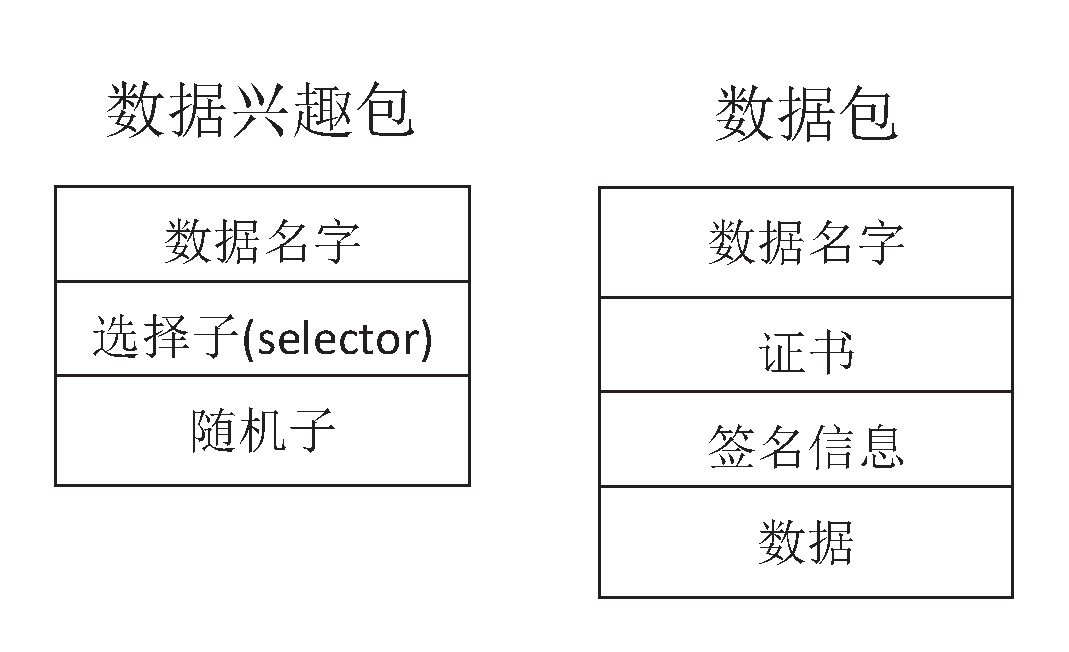
\includegraphics[width=0.7\textwidth]{NDN-packet}
  \caption{IP与NDN架构对比}
  \label{fig:NDN-packet}
\end{figure}

NDN协议处理架构主要是基于三个表即转发表(Forwarding Information Base,FIB),兴趣等待表(Pending Interest Table,PIT)与内容缓存(Content Store,CS)。FIB转发表类似于IP的转发表,用来存储名字前缀以及对应的转发接口。PIT表用来存储在本节点转发出去并且还没被相应的interest。CS表即内容缓存,用来缓存返回的数据包。

一个节点处理interest请求过程为,首先查找CS看是否有对应的数据包,如果有直接返回,如果没有则查找FIB表,看有没有转发的合适条目,如果存在则按照FIB规则转发,同时interest被存储在PIT中。当对应的请求包回到该节点时,一方面根据CS缓存策略对该数据包进行缓存,另一方面根据PIT表存储的interest信息返回该数据,并删除PIT表中的该条目。

\subsection{基于信息中心网络的服务网络相关研究}
ICN本质上是把传统网络中的\textit{where}模型转化为\textit{what}模型,网络直接处理的是应用数据的抽象。而一些研究在数据之上进一步地进行抽象,认为网络的本质是承载与连接服务。

文献\cite{nordstrom2012serval}提出一种服务中心网络协议栈(Serval)。通过ServiceID来标记应用网络包,通过FlowID用来标记当连接建立后的网络包。Serval协议栈中还增加了Service Table和Flow Table用来记录Service和Flow的网络状态,在Host端可以可以针对网络服务情况进行状态保持和只能决策。

文献\cite{braun2011service,braun2013service}中提出一种服务中心网络(Service-Centric Networking,SCN)架构以及一种基于NDN的服务中心网络实现。在沙漏架构中将NDN的命名数据包替换成服务对象。SCN修改Interest的结构使其能够封装服务请求参数。但整体来说SCN就是对NDN表述的重新抽象以及对流程的简单修改。

文献\cite{wu2014sofia}提出了一种基于ICN的面向服务信息网络架构(SOFIA)。而SOFIA的本质也是利用了NDN的命名、转发与缓存机制。此外在SOFIA中增加了Service Relay角色,相当于一种服务代理。服务请求者可以请求Service Relay在不同的网络环境中进行新的服务请求连接。这种机制有助于网络中multihoming,multicast以及mobility的实现。
